\documentclass[14pt,aspectratio=169, serif, dvipsnames]{beamer} 

%Beamer theme
\usetheme{Marburg}

%Packages
\usepackage[utf8]{inputenc} 
\usepackage[english]{babel}
\usepackage{graphicx}
\usepackage{amsmath}  
\usepackage{amsthm, thmtools}
\usepackage{braket} 
\usepackage{relsize}
\usepackage{float}
\usepackage{lmodern} % math, rm, ss, tt
\usepackage[T1]{fontenc}
\usepackage{fancyhdr}
% \usepackage[dvipsnames]{xcolor} %if uncommented will cause errors
\usepackage{framed}
\usepackage[normalem]{ulem}
\usepackage{tikz-cd}
\usepackage{tikz}
\usepackage[most]{tcolorbox}
\usepackage{bm}
\usepackage{old-arrows}
\usepackage[usestackEOL]{stackengine}
\usetikzlibrary{arrows}
\usetikzlibrary{arrows.meta}
\tikzcdset{arrow style = tikz, diagrams={>={Stealth[scale=1]}}}

%Math commands
\newcommand{\normal}{\unlhd}
\newcommand{\labelenumi}{{\bf (\alph{enumi})}} 
\renewcommand{\ker}{\mbox{Ker}}
\renewcommand{\hom}{\mbox{Hom}}
\renewcommand{\epsilon}{\varepsilon}
\renewcommand{\phi}{\varphi}
\renewcommand{\im}{\text{Im}}

%Backslash key not allowed in LaTeX, so we rename the command
\newcommand{\bs}{\textbackslash} %we write bs as short for "backslash"


%%%%%%%Slide titles
\author{Mengyi Shan, Luke Trujillo}

\newcommand{\TT}{Surface Representations of Sound} 

%Start of document
\begin{document}
\title{\TT}
\date{May 6, 2020} 
\titlepage

\small 

\section{Main Paper and Direction}
\begin{frame}{Surface Representations}
    In the paper we studied, the authors created created surfaces of spectrograms and implemented a time warping algorithm.
    \vspace{0.5cm}
    
    Given an audio signal $x(t)$, the authors first generated spectrograms by computing the \textbf{local Fourier transform}, given by
    \[
        X(\omega, t) = \int_{-\infty}^{\infty}x(t)\psi(\tau - t)\text{exp}(-j\omega \tau)d\tau   
    \]
    taken at frequency $\omega$ and time $t$
    using a Gaussian window function with size 10 milliseconds.
    \[
    \psi(\tau) = \text{exp}\left(-\frac{1}{2}\left(\frac{\tau}{0.5(10^{-0.2})}\right)^2\right).
    \]
\end{frame}

\begin{frame}{Surface Representations}
    The authors then computed the \textbf{power spectral density} of the signal:
    \[
        P(\omega, t) = 10\log_{10}(|X(\omega, t)|^2) 
    \]
    and created surface representations of sound by corresponding them 
    to the height functions $(t, \omega, P(\omega, t)$.
    \vspace{1cm}
    
    Spectrograms themselves are three dimensional surfaces projected to $\mathbb{R}^2$. 
    The authors are simply rescaling them in $\mathbb{R}^3$.
    However, this immediately leads to issues with noise and smoothing.

\end{frame}

\section{Smoothing Surfaces}

\begin{frame}{Smoothed PSD for "Potato"}
    \begin{center}
        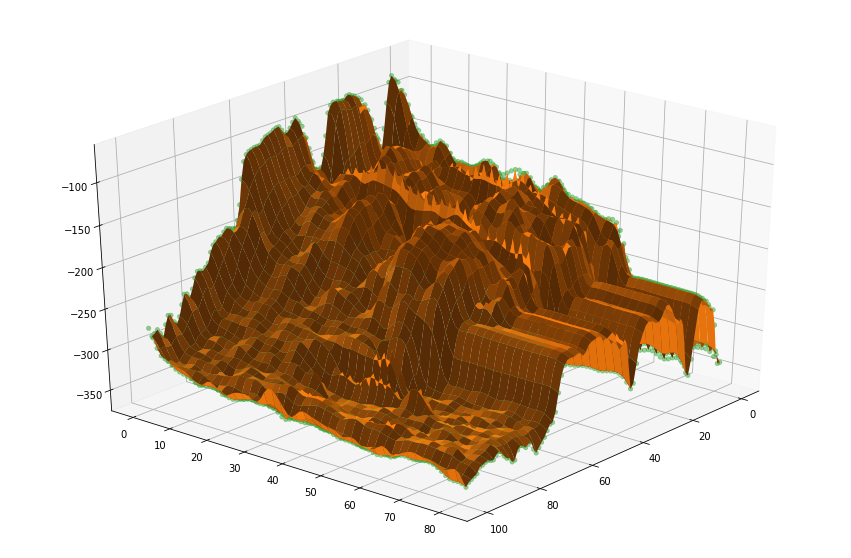
\includegraphics[scale = 0.4]{pictures/potato_psd.png}
    \end{center}
\end{frame}

\begin{frame}{Smoothed PSD for "Potato"}
    \begin{center}
        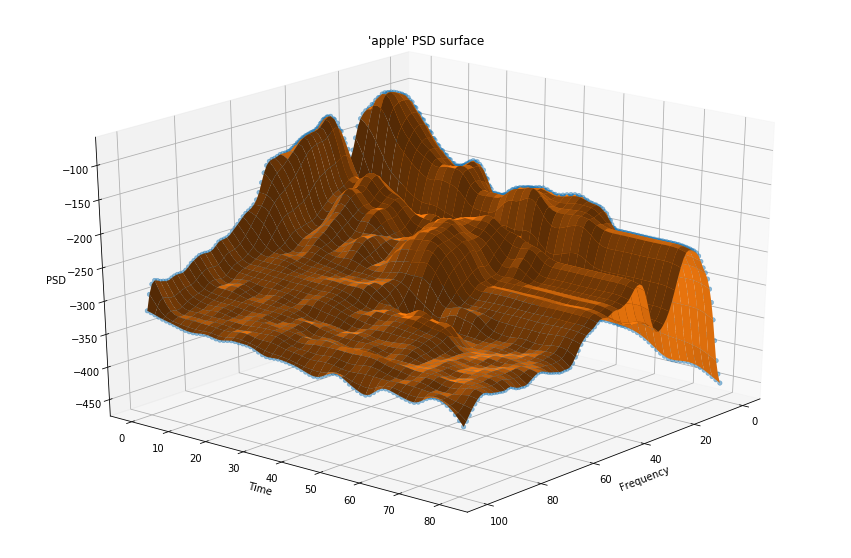
\includegraphics[scale = 0.4]{pictures/smoother_potato.png}
    \end{center}
\end{frame}

\begin{frame}{Smoothed PSD for "Apple"}
    \begin{center}
        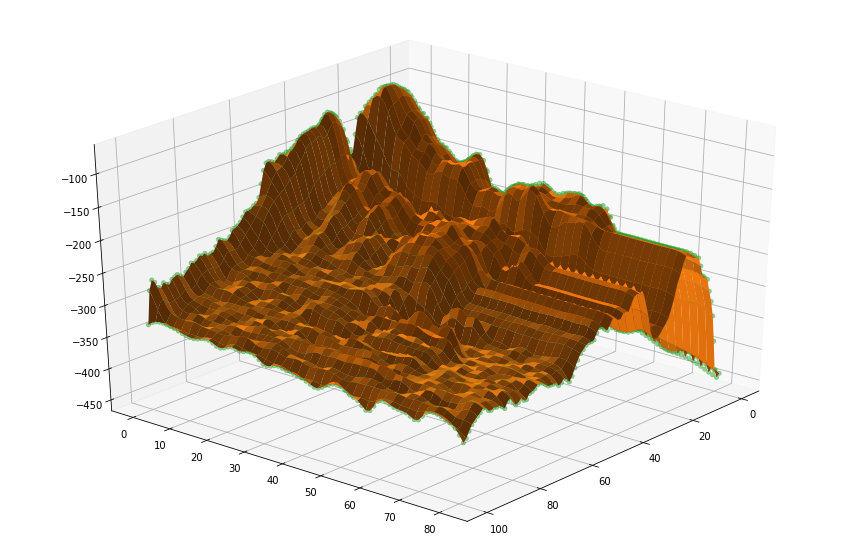
\includegraphics[scale= 0.4]{pictures/apple.png}
    \end{center}
\end{frame}

\begin{frame}{Smoothed PSD for "Apple"}
    \begin{center}
        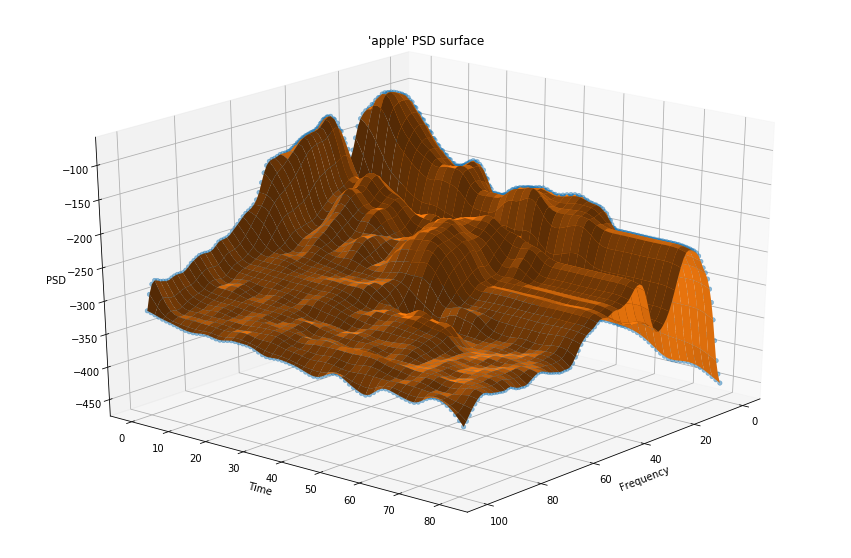
\includegraphics[scale= 0.4]{pictures/smoother_apple.png}
    \end{center}
\end{frame}

\begin{frame}{Smoothed PSD for "Monstrosity"}
    \begin{center}
        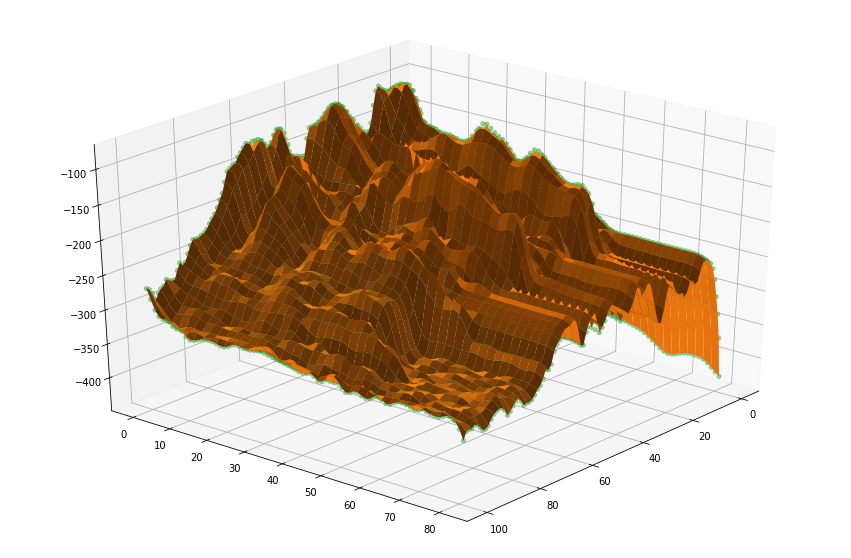
\includegraphics[scale=0.4]{pictures/monstrosity.png}
    \end{center}
\end{frame}

\begin{frame}{Smoothed PSD for "Monstrosity"}
    \begin{center}
        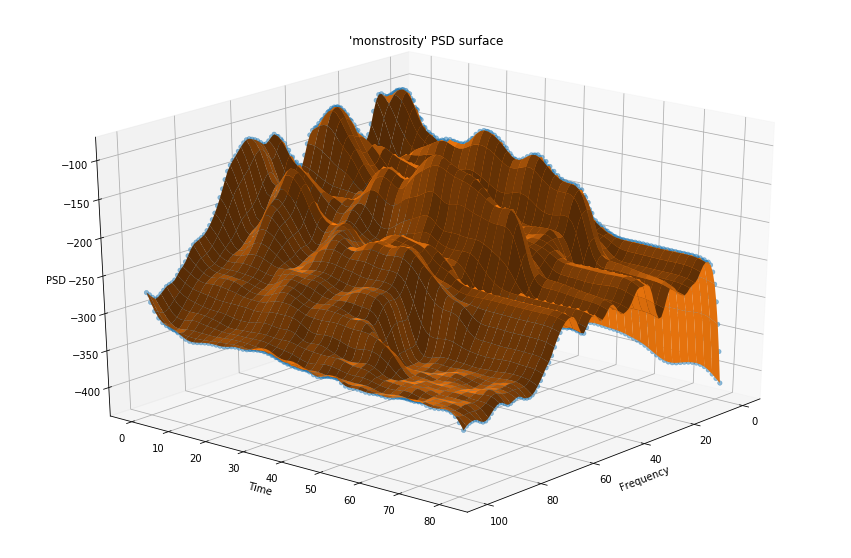
\includegraphics[scale=0.4]{pictures/smoother_monstrosity.png}
    \end{center}
\end{frame}

\section{Concatenating Surfaces}

\begin{frame}{Concatenating Surfaces}
    Concatenating surfaces is a difficult challenge, but it is simplified if we only scale along the time axis which helps preserve the information.
    \vspace{1cm}
    
    Peaks of our PSD surfaces are almost always located along the lowest frequency axis. Therefore we scaled our surfaces by aliging their maxima on these axes, while trying to avoid scaling too much. 
\end{frame}

\begin{frame}{Concatenating Surfaces}
The phonemes "u" and "p" concatenated together
\begin{center}
    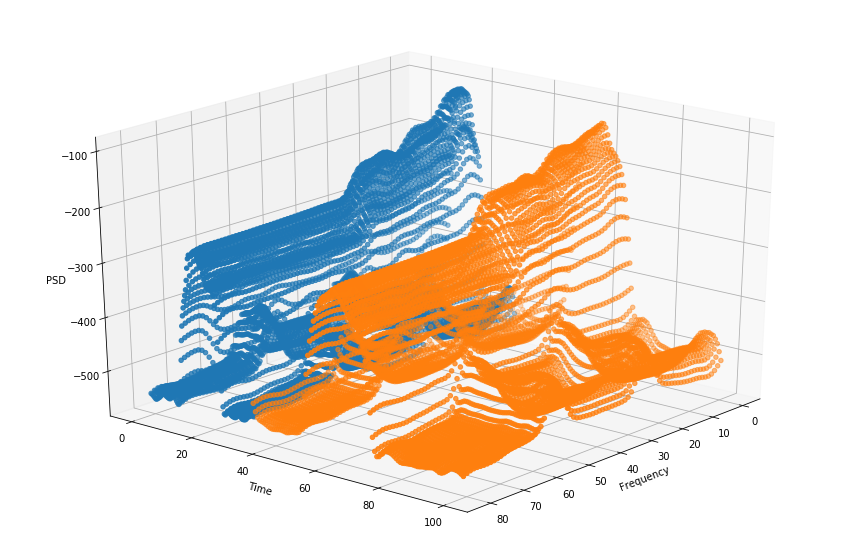
\includegraphics[width = 0.8\textwidth]{pictures/uh_p_plot.png}
\end{center}

\end{frame}

\begin{frame}{Concatenating Surfaces}
    The plot for the word "up", generated by phonemes 
    "u" and "p".
    \begin{center}
        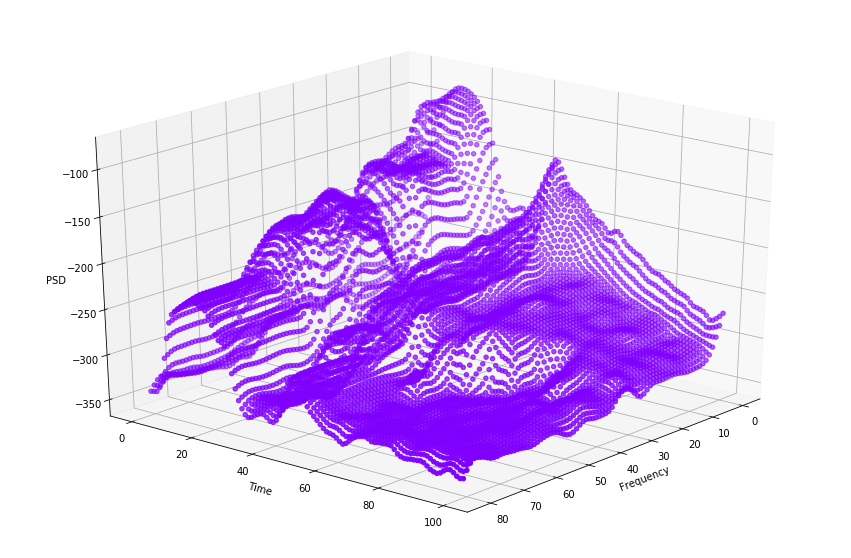
\includegraphics[width = 0.8\textwidth]{pictures/up_plot.png}
    \end{center}
\end{frame}

\begin{frame}{Concatenating Surfaces}
Concatenation of the phonemes "k" and "a:" (sounds like "are")
    \begin{center}
        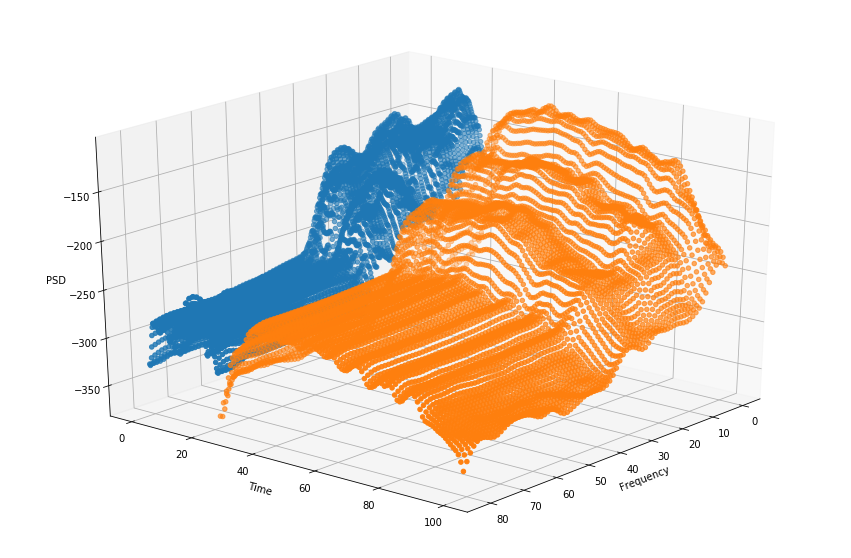
\includegraphics[width = 0.8\textwidth]{pictures/k_ar_plot.png}
    \end{center}
\end{frame}

\begin{frame}{Concatenating Surfaces}
The plot of the word "car" made of phonemes "k" and "a:".
    \begin{center}
        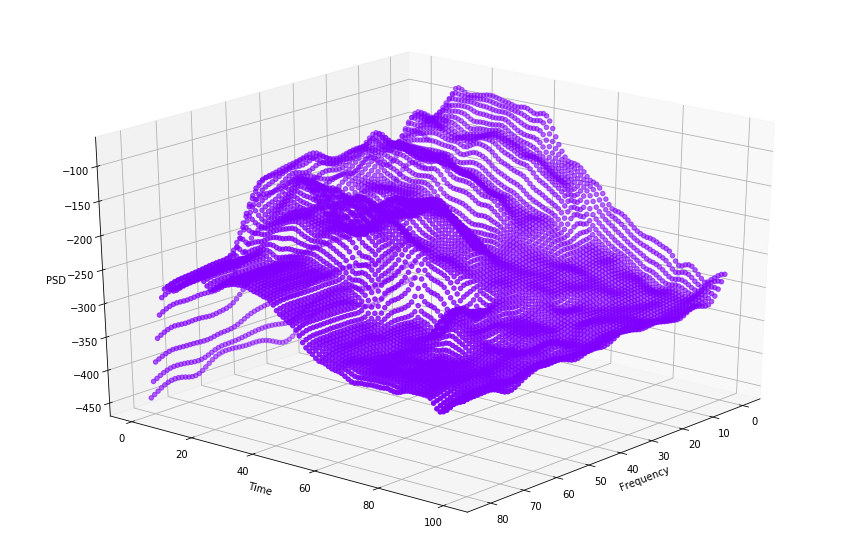
\includegraphics[width = 0.8\textwidth]{pictures/car_test_plot.png}
    \end{center}
\end{frame}
    

\small \section{Persistence Homology}
\begin{frame}{Persistence Homology}
    Let $X$ be a topological space. Consider the $n$-th homology
    group
    \[
        H_n(X)
    \]
    and suppose that $f: X \to \mathbb{R}$ is a real-valued function. For  any $a \in \mathbb{R}$, consider the topological space
    \[
        f^{-1}((\infty,a]) \subset X
    \]
    which inherits the subspace topology from $X$.
    Observe that
    if $a \le b$ then this induces a function 
    \[
        i: f^{-1}((\infty, a]) \to f^{-1}((\infty, b])
    \]
    namely, the inclusion function.
\end{frame}

\begin{frame}{Persistence Homology}
    Now consider the homology group of this subspace
    \[
        H_n(f^{-1}((\infty, a]))
    \]
    and observe that for any $a \le b$,
    we have a group homomorphism which we denote as $\phi_a^b$:
    \[
        \phi_a^b: H(f^{-1}(\infty, a]) \to H(f^{-1}(\infty, b]).
    \]
    What we've created is a functorial data pipeline
    \begin{align*}
        a \longmapsto f^{-1}((\infty, a]) \longmapsto H(f^{-1}((\infty, a])).
    \end{align*}
    which sends numbers to topological spaces to abelian groups. 
    What this records is the evolution of the homology of our function defined on the topological space!
\end{frame}

\begin{frame}{Persistence Homology}
    An example of this pipeline is if $X$ is a sphere and $f: X \to \mathbb{R}$ is the height function. 
    \begin{center}
    \scalebox{0.7}{
        \begin{tikzpicture}
        \filldraw[orange, opacity = 0.2] (0,0) circle (3) ;
    
        \draw[dashed] (3,0,0) arc (0:90:3);
        \draw[dashed] (3,0,0) arc (0:360:3);
        \filldraw[color=orange!10] (3,0) arc (0:-180:3cm and 15mm) arc (180:0:3cm and 3cm);
    
        \draw[thick] (0,0) circle (3) ;
        \path[draw,dashed] (3,0) arc [start angle=0, end angle=180,
        x radius=3cm,
        y radius=1.4cm] ;
        \path[draw] (-3,0) arc [start angle=180, end angle=360,
            x radius=3cm,
            y radius=1.5cm] ;
        
        % real line
        \draw[thick, {Triangle}-{Triangle}] (7,-3) -- (7,3);
        \draw[thick, Orange] (7, -2) -- (7, -0.5);

        % tick marks
        \draw (6.75,2) -- (7.25,2);
        \draw (6.75,-0.5) -- (7.25,-0.5);
        \draw (6.75,-2) -- (7.25,-2);

        % labels
        \node at (7.7, -2) {0};
        \node at (7.7, -0.5) {$a$};
        \node at (7.7, 2) {1};
        \node at (5, 0.8) {$f^{-1}((-\infty, a])$};

        % arrow
        \draw[-{Triangle}] (6.5, -0.2) to [bend right] (3.5, -0.2);
    \end{tikzpicture}
    }
    \end{center}  
    As $a$ increases, we can keep track of the homology groups to understand our data better. 
    
    But, for nice spaces (e.g. simplicial complexes), the homology usually won't change much. 
\end{frame}

\begin{frame}{Persistence Homology}
    What we mean is that, in general, 
    \[
        \phi_a^b: H(f^{-1}(\infty, a]) \to H(f^{-1}(\infty, b]).
    \]
    is usually an isomorphism. Therefore we define
    \begin{align*}
        \beta_a^{b}
        &=
        \text{rank}(\im(\phi_a^b))\\
        &=
        \text{rank}(\im\Big( H(f^{-1}((\infty, a ])) \to H(f^{-1}((\infty, b])) \Big))
    \end{align*}
    to be the \textbf{Betti number from $a$ to $b$} and we pay attention to whether or not this number changes.
\end{frame}

\begin{frame}{Persistence Homology}
    Moreover, if we do find an $a$ such that, for some $\epsilon$, the homomorphism
    \[
        H_n(f^{-1}((\infty, a - \epsilon])) \to H_n(f^{-1}((\infty, a +\epsilon ]))
    \]
    is \emph{not} an isomorphism, then we say $a$ is a \textbf{critical value}. This means something happened to our homology; i.e., a singularity (like a hole or a vertex) was 
    encountered. 
    \vspace{0.5cm}
    
    Researchers were aware of this pipeline for sometime, but it was only in the 2000's that applied topologists created an extremely useful and stable tool for efficiently utilizing this technology.
\end{frame}

\begin{frame}{Persistence Homology}
    Suppose we have finitely many critical values $\{s_1, s_2, \dots, s_n\}$.
    Let $\{t_0, t_1, \dots, t_{n}\}$ be any interleaved sequence of numbers such that $t_{i-1} < s_i < t_{i}$.
    \vspace{0.5cm}
    
    Let $f: X \to \mathbb{R}$ have finitely many critical values
    and let
    $(s_i, s_j)$ be a tuple of critical values. Then we define the \textbf{multiplicity} 
    of $(s_i, s_j)$ to be
    \[
        \mu_{i}^{j} = \beta_{t_{i-1}}^{t_i} -\beta_{b_i}^{b_j} + \beta_{b_{i}}^{b_{j-1}} - \beta_{b_i}^{b_j}
    \]
\end{frame}

\begin{frame}{Persistence Homology}
    The persistence diagram of the tame function $f: X \to \mathbb{R}$, denoted
    $D(f)$, is the \emph{multiset} of tuples $(s_i, s_j)$ each with multiplicity $\mu_i^j$.
    
    \begin{center}
        \scalebox{0.8}{
    \begin{tikzpicture}
        % Outer background color
        \filldraw[Yellow!15] (-3, -2) -- (-3,5.5) -- (5.5, 5.5) -- (5.5,-2) -- cycle;

        % Axes
        \def\axeslen{5}
        \draw[thick, {Triangle}-{Triangle}, Black!60] (-1, 0) -- (\axeslen, 0);
        \draw[thick, {Triangle}-{Triangle}, Black!60] (0, -1) -- (0, \axeslen);
        \draw[thick, -{Triangle}] (0,0) -- (4,4);

        % vertical lines
        \draw[-{Triangle}] (1,1) -- (1, 4);
        \draw[-{Triangle}] (2,2) -- (2, 4);
        \draw[-{Triangle}] (3,3) -- (3, 4);

        %horizontal lines
        \draw[-{Triangle}] (1,1) -- (-2, 1);
        \draw[-{Triangle}] (2,2) -- (-2, 2);
        \draw[-{Triangle}] (3,3) -- (-2, 3);

        % The labels
        \node at (4.7,-0.3){$x$};
        \node at (-0.3,4.7) {$y$};
        \node at (1, -0.4) {$s_1$};
        \node at (2, -0.4) {$s_2$};
        \node at (3, -0.4) {$s_3$};

        % The tickmarks
        \draw[Orange] (1, -0.1) -- (1, 0.1);
        \draw[Orange] (2, -0.1) -- (2, 0.1);
        \draw[Orange] (3, -0.1) -- (3, 0.1);

        \draw[NavyBlue!80] (0.5, -0.05) -- (0.5, 0.05);
        \draw[NavyBlue!80] (1.5, -0.05) -- (1.5, 0.05);
        \draw[NavyBlue!80] (2.5, -0.05) -- (2.5, 0.05);
        \draw[NavyBlue!80] (3.5, -0.05) -- (3.5, 0.05);

        % circles
        \filldraw[Orange] (1,1) circle (0.25ex);
        \filldraw[Orange] (2,2) circle (0.25ex);
        \filldraw[Orange] (3,3) circle (0.25ex);
        \filldraw[Orange] (1,2) circle (0.25ex);
        \filldraw[Orange] (1,3) circle (0.25ex);
        \filldraw[Orange] (2,2) circle (0.25ex);
        \filldraw[Orange] (2,3) circle (0.25ex); 
        \filldraw[Orange] (3,3) circle (0.25ex);

        \filldraw[NavyBlue!80] (0.5,0.5) circle (0.2ex);
        \filldraw[NavyBlue!80] (0.5,1.5) circle (0.2ex);
        \filldraw[NavyBlue!80] (0.5,2.5) circle (0.2ex);
        \filldraw[NavyBlue!80] (0.5,3.5) circle (0.2ex);
        \filldraw[NavyBlue!80] (1.5,1.5) circle (0.2ex);
        \filldraw[NavyBlue!80] (1.5,2.5) circle (0.2ex);
        \filldraw[NavyBlue!80] (1.5,3.5) circle (0.2ex);
        \filldraw[NavyBlue!80] (2.5,2.5) circle (0.2ex);
        \filldraw[NavyBlue!80] (2.5,3.5) circle (0.2ex);
        \filldraw[NavyBlue!80] (3.5,3.5) circle (0.2ex);

    \end{tikzpicture}
    }
    \end{center}
\end{frame}

\begin{frame}{Persistence Homology}
    In recent years, persistence homology has become an extremely useful tool for time-series analysis. Given a dataset, a sliding window embedding can be performed to create a point-cloud:
    
    \begin{center}
        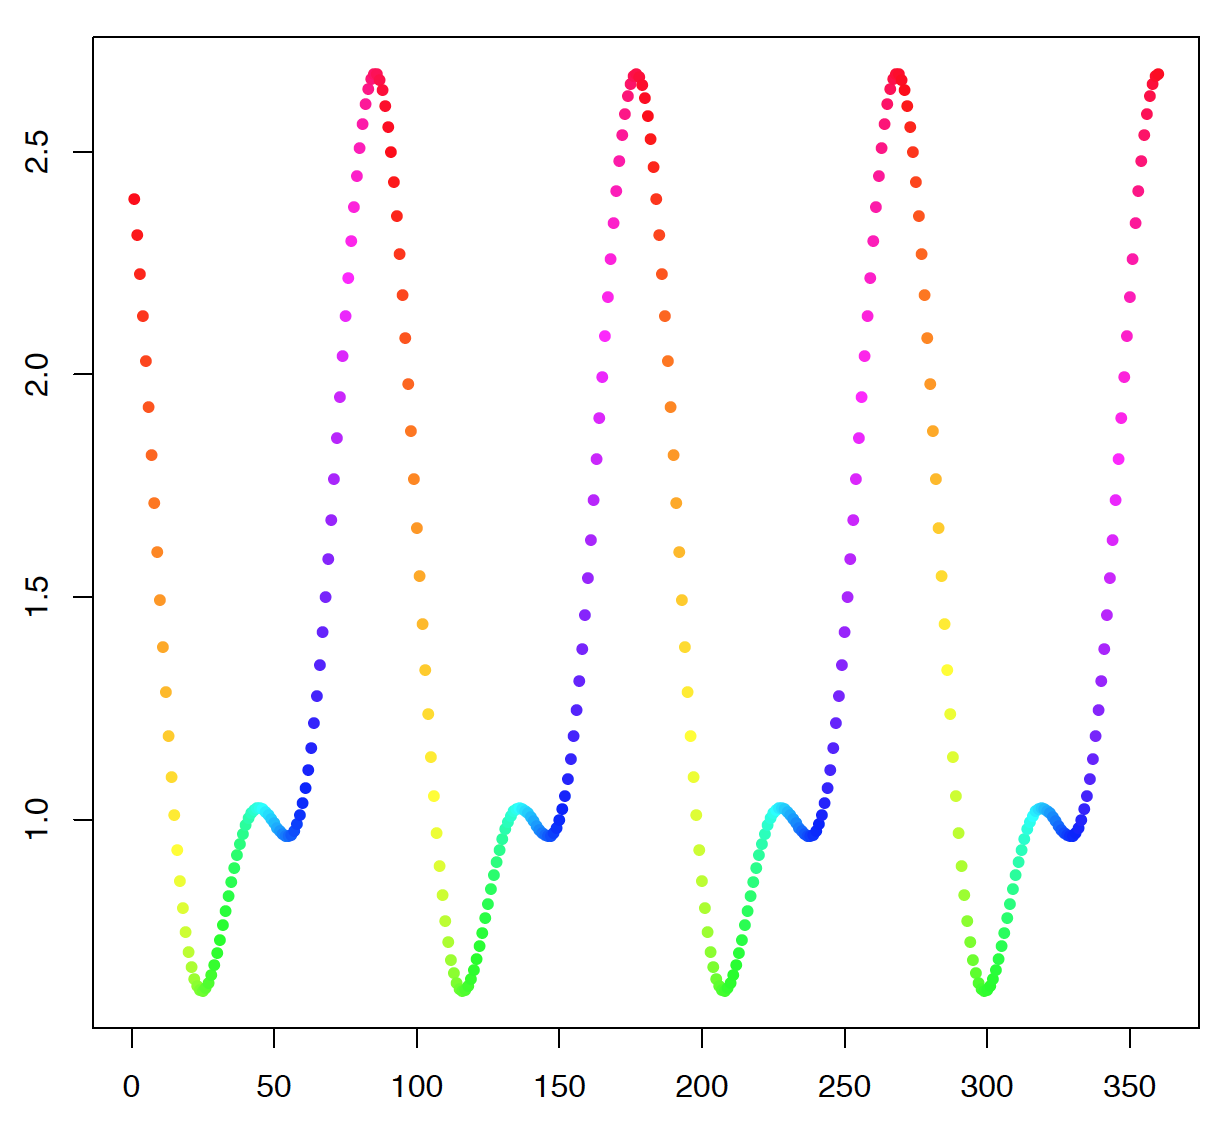
\includegraphics[width =         0.4\textwidth]{pictures/TimeSeries.png}
        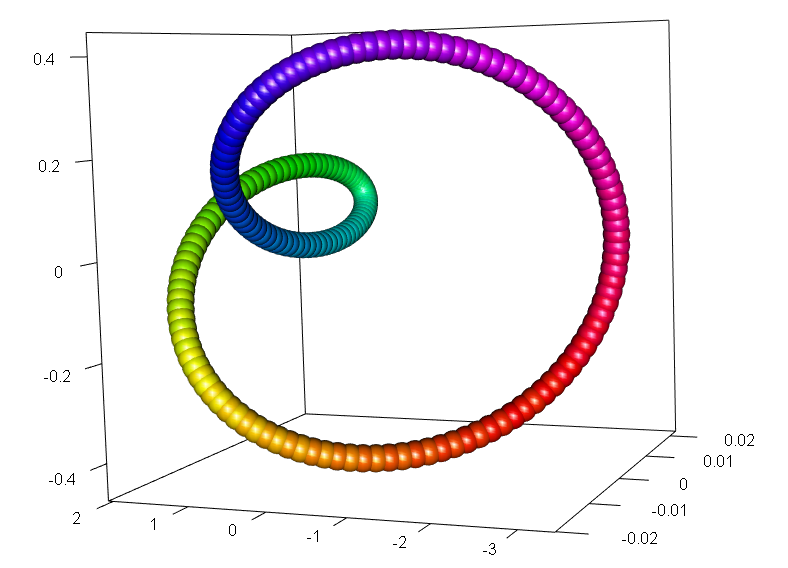
\includegraphics[width = 0.5\textwidth]{pictures/pointcloud.png}
    \end{center}
    
    The homology of the resulting object is then studied.
\end{frame}

\begin{frame}{Persistence Homology}
    In the case of real data, the homology of the data is filtered as a simplicial complex.
    
    \begin{center}
        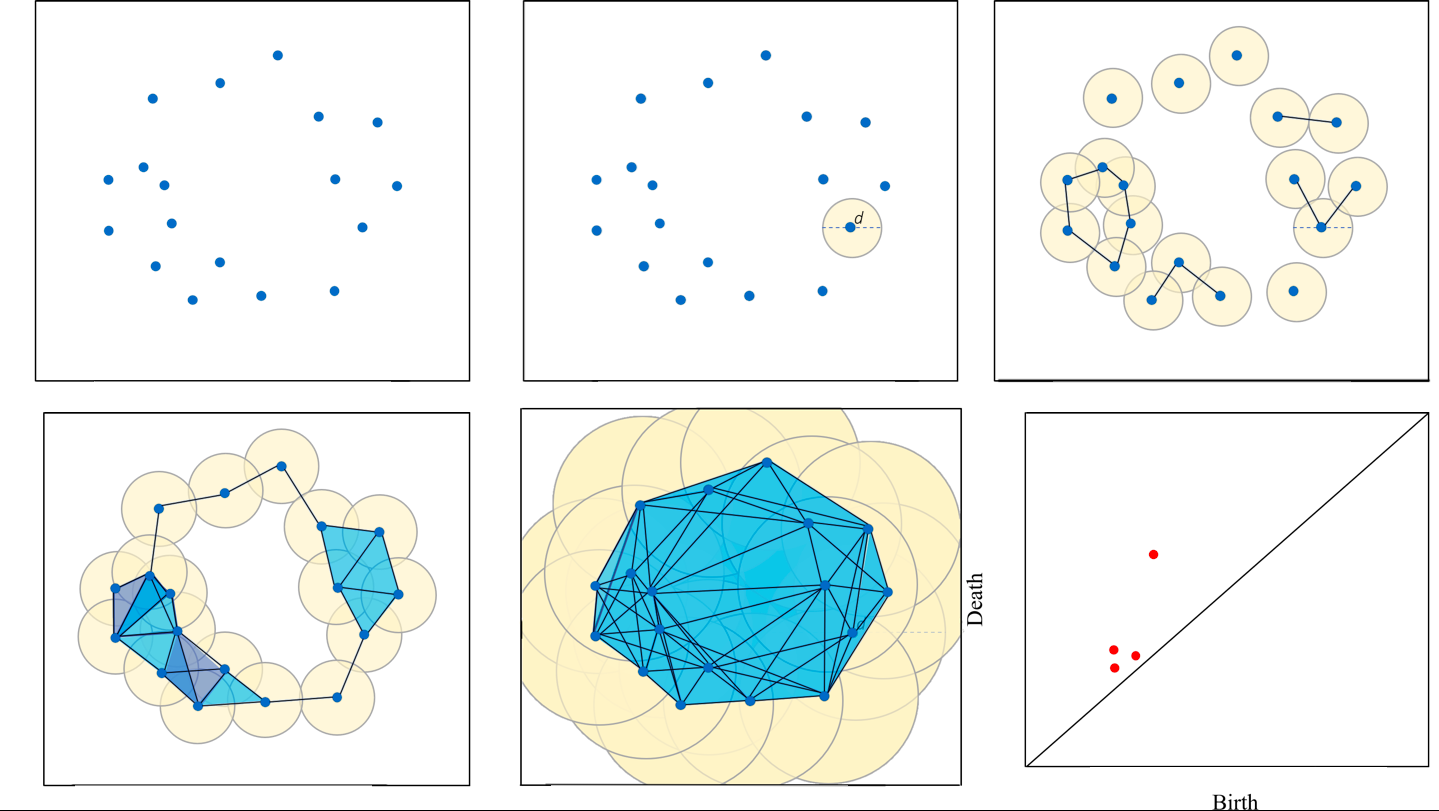
\includegraphics[width = 0.7\textwidth]{pictures/filtration.png}
    \end{center}
    
    The most popular filtration is the Vietoris-Rips, which we used in our project.
\end{frame}



\section{Coding}
\begin{frame}{Coding}
    \begin{itemize}
        \item  We utilized the GUDHI (Geometric Understanding 
        in Higher Dimensions) python package for the project
    
        \item Used $\mathbb{Z}_2$ homology, which is fast and also intuitive
        
        \item We filted our data using the Vietoris Rips complex. 
    \end{itemize}
\end{frame}

\begin{frame}{Vowels}
    There is a significant difference in the persistence diagrams between vowels and consonants: 
    \begin{center}
        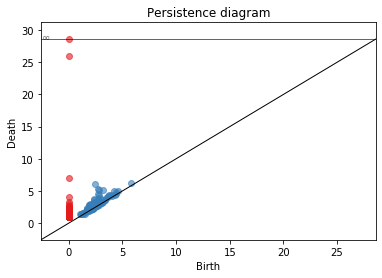
\includegraphics[width = 0.5\textwidth]{pictures/k_pers_plot.png}
        \hspace{-0.6cm}
        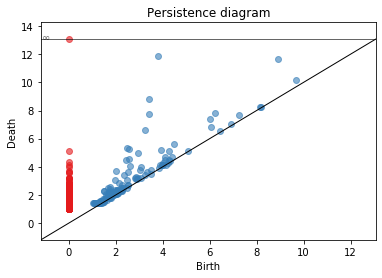
\includegraphics[width = 0.5\textwidth]{pictures/ar_pers_plot.png}
    \end{center}
    The above left is for the phoneme "k" 
    while the one on the right is for the phoneme "a:" (sounds like the word "are").
\end{frame}

\begin{frame}{Vowel Strength}
    The difference is also apparent when considering words with vowels of different strengths. 
        \begin{center}
        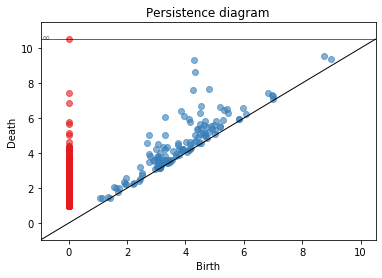
\includegraphics[width = 0.5\textwidth]{pictures/no_pers_plot.png}
        \hspace{-0.6cm}
        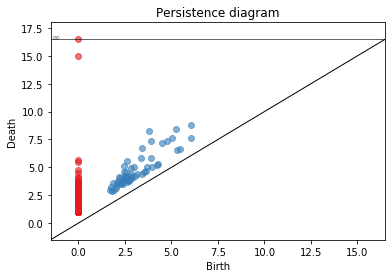
\includegraphics[width = 0.5\textwidth]{pictures/yes_pers_plot.png}
    \end{center}
    The above left is the word "no", which has a strong vowel, while the one of the right is "yes", which is weaker.
\end{frame}

\begin{frame}{Rhymes}
    We also checked words that rhyme to see if their persistence diagrams are similar. 
    \begin{center}
        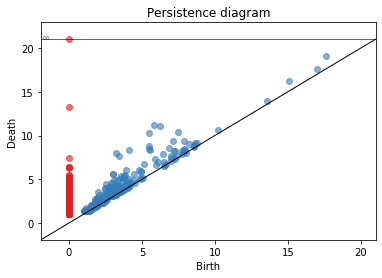
\includegraphics[width = 0.5\textwidth]{pictures/tarnation_pers_plot.png}
        \hspace{-0.6cm}
        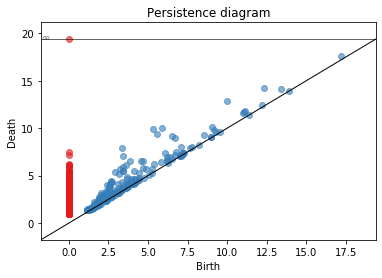
\includegraphics[width=0.5\textwidth]{pictures/vacation_pers_plot.png}
    \end{center}
    The above left is the word "tarnation", while the above right is for the word "vacation."
\end{frame}


\end{document}